\section{Техническое задание}
\subsection{Основание для разработки}

Полное наименование системы: <<Веб-приложение \textquotedbl Социомаркет для владельцев домашних животных \textquotedbl\ >>.
Основанием для разработки программы является приказ ректора ЮЗГУ от <<24>> ноября 2023 г. №5166-с <<Об утверждении тем выпускных квалификационных работ>>.

\subsection{Цель и назначение разработки}

Веб-приложение <<Социомаркет для владельцев домашних животных>> создается с целью объединения пользователей двух групп: владельцев домашних животных и лиц, предоставляющих услуги для домашних животных. Такими лицами могут являться владельцы интернет-магазинов, предприниматели или такие же пользователи.

Задачами данной разработки являются:
\begin{itemize}
\item создание каталогов с категориями карточек на сайте;
\item разработка клиентской части web-сайта;
\item создание каталогов с категориями карточек на сайте;
\item реализация формы создания и управления карточкой услуги;
\item создание удобного поиска по каталогам карточкам;
\item реализация взаимодействия между пользователями сайта;
\item разработка и развертывание инфраструктуры web-сайта и его базы данных на удаленном сервере;
\item разработка серверной части web-сайта;
\item разработка REST API для взаимодействия клиентской и серверной частей;
\item разработка базы данных.
\end{itemize}

Задачей разработки серверной части так же является следования принципам, описанным в работе Марка Прайса <<C\# 9 и .NET 5. Разработка и оптимизация>>~\cite{mark_price}.

\subsection{Требования пользователя к интерфейсу web-сайта}

Сайт должен включать в себя:
\begin{itemize}
    \item авторизацию;
    \item навигацию по разделам;
    \item разделение доступа к функционалу сайта для пользователя и лица предоставляющего услуги;
    \item поиск по пользователям и их товарам или услугам.
\end{itemize}


\subsection{Требования к программной системе веб-приложения <<Социомаркет>>}
\subsubsection{Требования к данным программной системы}
Система должна уметь эффективно обрабатывать данные пользователей, включая личную информацию, данные о питомцах, информацию о продуктах (товары и услуги). Необходимо обеспечить конфиденциальность и безопасность этих данных.
На рисунке ~\ref{bd:image} представлена концептуальная модель данных программной системы в виде UML-диаграммы сущность-связь.

\begin{figure}[ht]
\centering
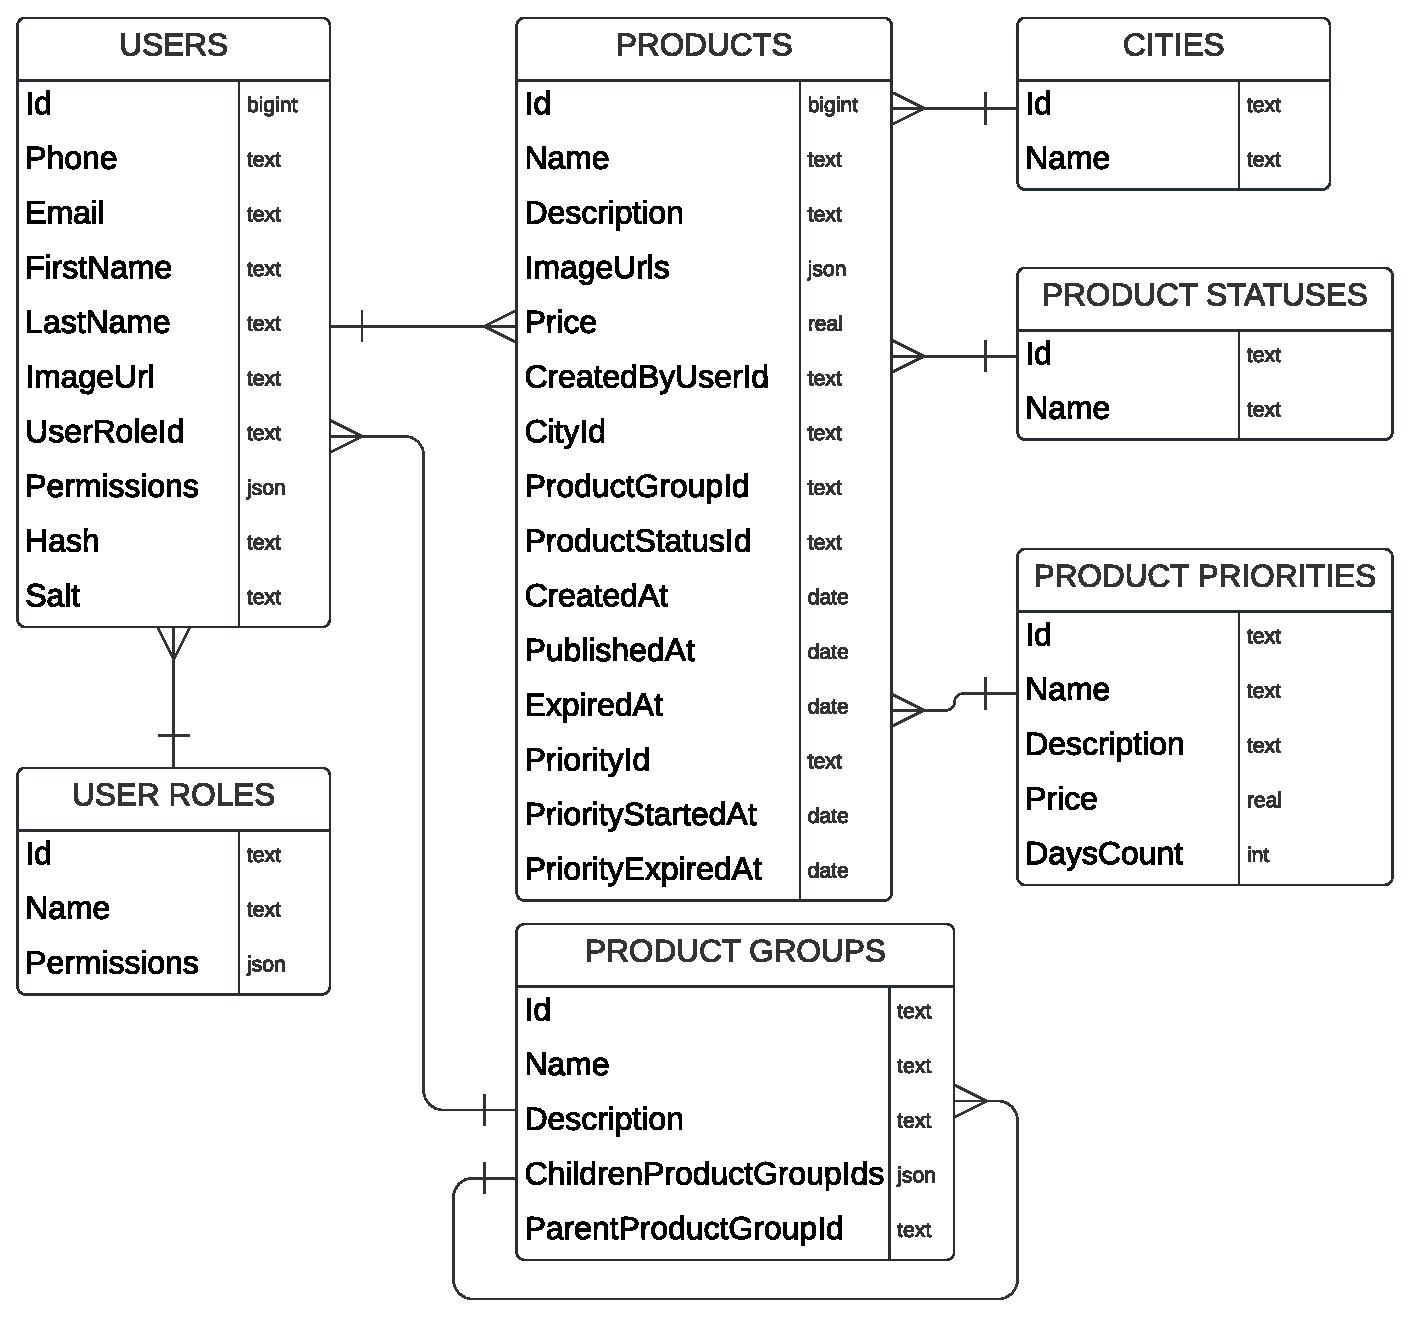
\includegraphics[width=1\linewidth]{bd}
\caption{Концептуальная модель данных}
\label{bd:image}
\end{figure}

В приведенной на рисунке ~\ref{bd:image} диаграмме сущность-связь представлены сущности и атрибуты, которые будут использоваться в программной системе.

Данные программной системы должны быть организованы таким образом, что бы не разделять на 2 отдельные группы пользователей и лиц, предоставляющих услуги. Отличие между пользователями должно быть записано в атрибуте <<UserRole>> сущности <<User>>. Таким образом, в программной системе будет только одна сущность <<User>>, которая будет иметь атрибут <<UserRole>> со значениями <<SITTER>> и <<OWNER>>.
При проектировании модели данных так же необходимо ущесто то, что сущность <<Product>> представляет собой продукт, который может быть как товаром, так и услугой. Для этого не требуется никаких дополнительных атрибутов, так как сущность <<Product>> становится товаром или услугой в зависисмости от названия и описания карточки продукта.

\subsubsection{Функциональные требования к программной системе}
В разрабатываемой программно-информационной системе должно быть предусмотрено наличие двух классов пользователей: владельцев домашних животных и лиц, предоставляющих услуги или товары для них.

\subsubsection{Архитектура системы} 
Серверная часть веб-приложения <<Социомаркет>> разработана на .NET Core, что отражает современные подходы в разработке программного обеспечения, описанные в <<C\# 9 и .NET 5. Разработка и оптимизация>>~\cite{mark_price}. Клиентская часть, реализованная на Angular, взаимодействует с сервером через REST API. База данных построена на PostgreSQL и соответствует рекомендациям и методикам, изложенным в документации PostgreSQL~\cite{postgresql}.

\subsubsection{Вариант использования <<Авторизация пользователя>>} 
Пользователи входят в систему, используя свой логин и пароль. Предусмотрена возможность восстановления пароля через электронную почту.

\subsubsection{Вариант использования <<Авторизация лица предоставляющего услуги>>}
Поставщики услуг и товаров регистрируются в системе, предоставляя специфическую информацию о предлагаемых услугах или товарах.

\subsubsection{Вариант использования <<Поиск>>} 
Пользователи могут искать продукты которые могут быть как товарами так и услугами, используя ключевые слова и фильтры для уточнения результатов. LINQ-запросы для выполнения поисковых операций.

\subsubsection{Вариант использования <<Просмотр каталогов карточек с товарами и услугами>>}
Пользователи могут просматривать карточки продуктов (товаров и услуг) в каталоге. Каждая карточка содержит информацию о товаре или услуге, включая описание, цену, фотографии и отзывы. Карточки можно фильтровать по категориям или тегам.

\subsubsection{Вариант использования <<Управление своими карточками>>}
Поставщики услуг и товаров могут создавать, редактировать и удалять свои карточки в каталоге. Это включает добавление описаний, цен, фотографий и другой релевантной информации.

\subsubsection{Вариант использования <<Инициировать обмен контактами между пользователями>>} 
Возможность отправить запрос на социальные сети другого пользователя для дальнейшего общения и сотрудничества.

\subsubsection{Вариант использования <<Редактирование профиля пользователя>>}
Пользователи могут редактировать свои личные данные, контактную информацию, а также настройки уведомлений и конфиденциальности.

\subsubsection{Вариант использования <<Просмотр профилей поставщиков услуг>>}
Пользователи могут просматривать профили поставщиков, включая описание услуг, фотографии и отзывы клиентов.

\subsubsection{Вариант использования <<Мобильная версия приложения>>}
Мобильная версия приложения обеспечивает удобство использования на смартфонах и планшетах, адаптируя интерфейс под мобильные устройства.

\subsubsection{Диаграмма прецедентов}
На рисунке ~\ref{people:image} представлена диаграмма прецедентов.

\begin{figure}[ht]
\centering
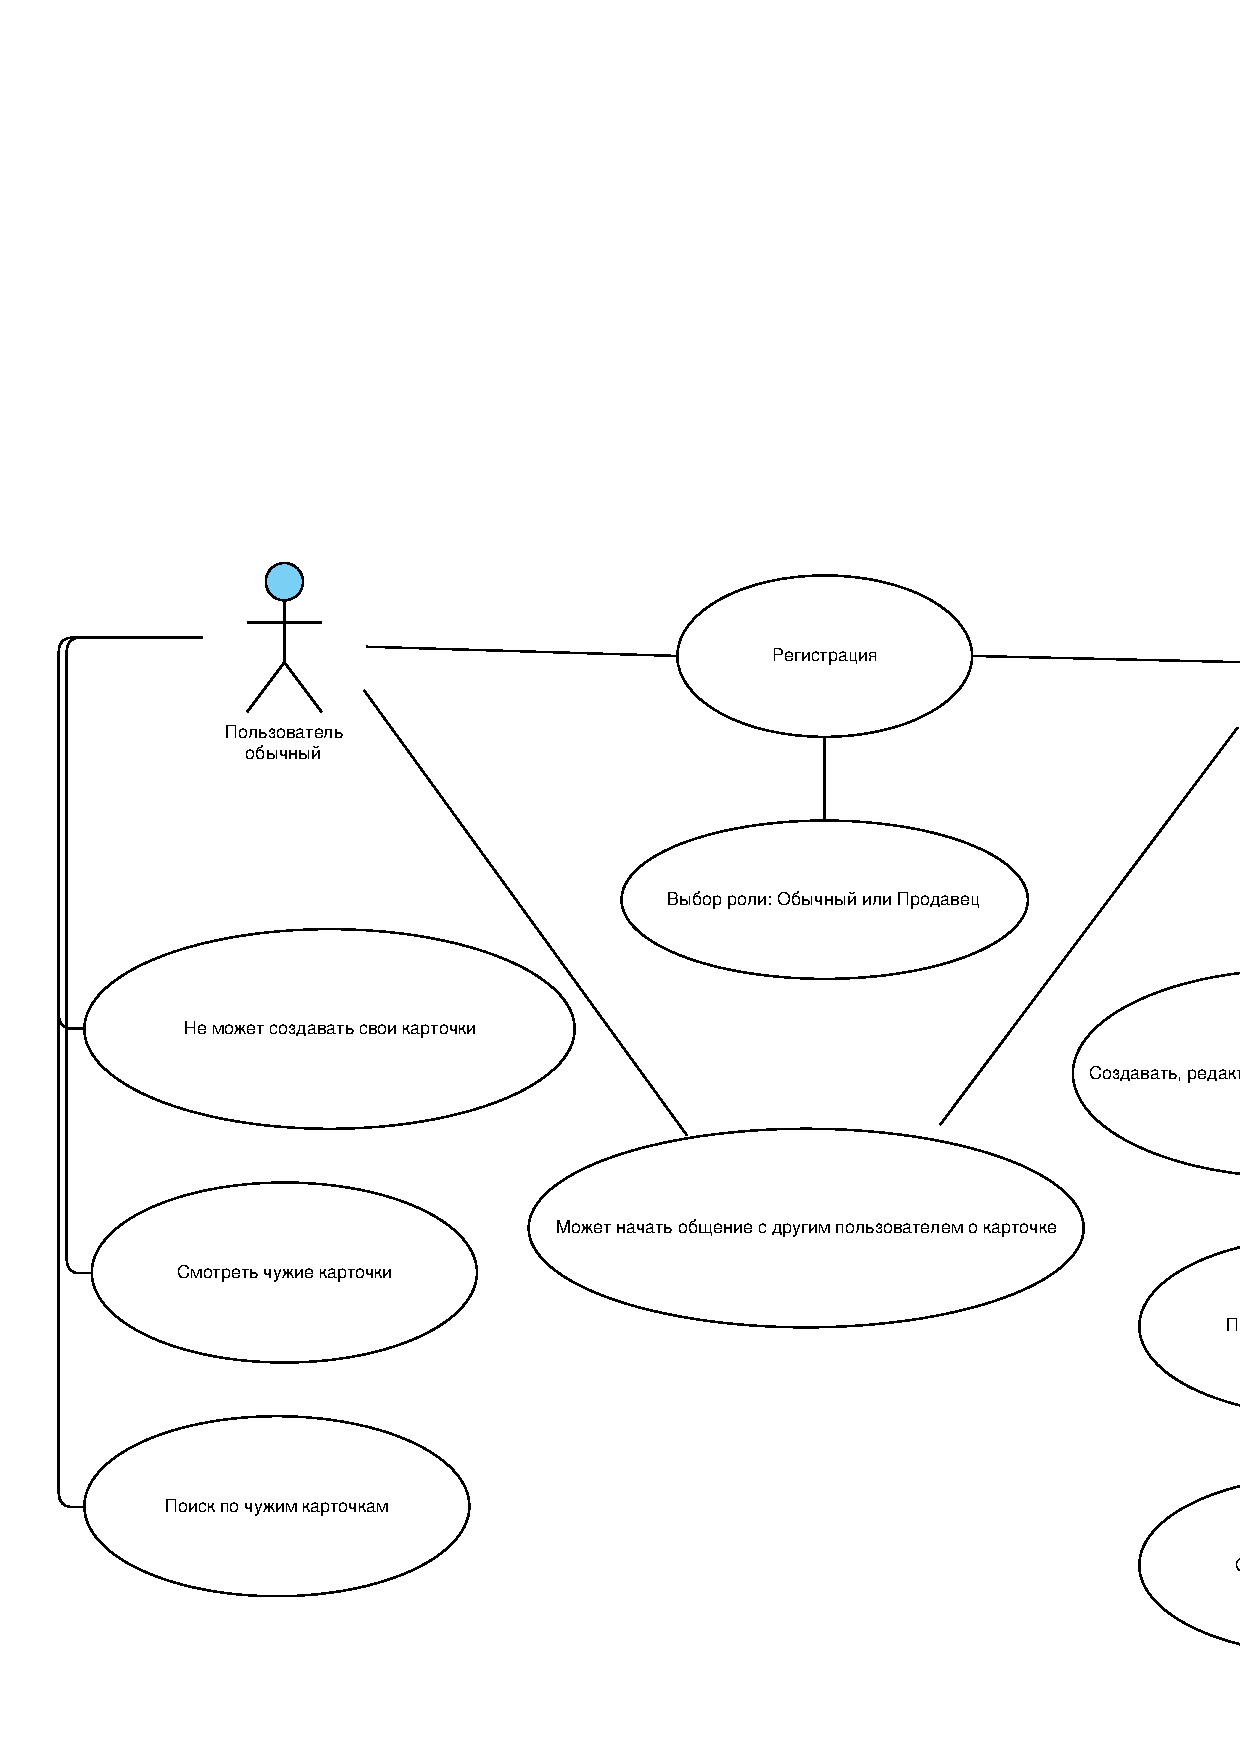
\includegraphics[width=1\linewidth]{people}
\caption{Диаграмма прецедентов}
\label{people:image}
\end{figure}

\subsection{Требования пользователя к интерфейсу приложения}
Интерфейс должен быть интуитивно понятным, удобным для пользователя, с четкой навигацией и адаптивным дизайном, подходящим для различных устройств. Принципы разработки интерфейса и адаптивного дизайна основаны на спецификациях HTML и CSS, как указано в <<Спецификация CSS>>~\cite{cssspecs} и <<Спецификация HTML>>~\cite{htmlbook}.
При проектировании интерфейса следует отказаться от диалоговых окон для крупных элементов сайта. То есть регистрация, поиск, результат поиска - все они будут на отдельных страницах, а не внутри диалоговых окон.

\subsection{Нефункциональные требования к программной системе}

\subsubsection{Требования к надежности}
В процессе работы серверной части программной системы возможны следующие аварийные ситуации:
\begin{enumerate}
\item Потеря доступа к сети Интернет;
\item Аварийное отключение электропитания;
\item Сбой операционной системы сервера.
\end{enumerate}

Для минимизации вероятности возникновения аварийных событий серверные компоненты программной системы должны быть размещены на выделенных серверах в дата-центрах хостинг-провайдеров, прошедших сертификацию и имеющих гарантию SLA>99,8\%. Операционная системадолжна получать регулярные накопительные обновления.

\subsubsection{Требования к безопасности}
Наличие механизма проверки целостности приложения путем использования криптографических функций, основанных на подписи пакета программы. Коммуникация с сервером по защищенному протоколу.

Требования к безопасности серверной части программной системы:
\begin{enumerate}
\item Регулярные обновления компонентов безопасности операционной системы;
\item Автоматическое обновление HTTPS-сертификатов;
\item Доступ к серверу должен осуществляться без разглашения IP-адреса целевой машины в целях предотвращения возможных атак типа DDoS;
\item Запросы к серверу должны предварительно обрабатываться на одельной машине с запущенным экземпляром сервера Nginx для контроля количества запросов и логирования обращений к серверу;
\item Правилами брандмауэра операционной системы основного сервера должно быть разрешено подключение к порту сервера только с IP-адреса промежуточной машины.
\end{enumerate}

Требования к безопасности клиентской части программной системы:
\begin{enumerate}
\item Поддержка современных браузеров и операционных систем, обеспечивающая стабильную и безопасную работу на различных платформах;
\item Использование технологий адаптивной верстки приложения;
\item Реализация защиты от XSS и CSRF атак, предотвращающая нежелательное вмешательство в работу приложения;
\item Регулярное обновление компонентов системы для предотвращения уязвимостей, связанных с устаревшим программным обеспечением.
\end{enumerate}

\subsubsection{Требования к программному обеспечению}
Для реализации программной системы должны быть использованы следующие языки программирования:
С\# -\- серверная часть приложения;
Type-script -\- клиентская часть приложения;
SQL -\- язык структурированных запросов к базе данных.

Для работы клиентской части приложения требуется ОС Android 5.0 или более поздняя версия или Windows 7 или более поздняя версия с установленным браузером Google Chrome.
Для работы серверных компонентов требуется ОС Windows 7 или Macos 12.0 или Ubuntu 16.0 или более поздняя версия c установленной СУБД PostgreSQL, .NET CORE 6.0, .NET SDK 6.0.

\subsubsection{Требования к аппаратному обеспечению}
Для сервера необходим центральный процессор с количеством ядер от 6 и выше с частотой ядра от 2.4 ГГц. Объем оперативной памяти – 32 Гб. Требование к скорости интернет-соединения – 100 Мбит/c и выше.

\subsection{Требования к оформлению документации}
Требования к стадиям разработки программ и программной документации для вычислительных машин, комплексов и систем независимо от их назначения и области применения, этапам и содержанию работ устанавливаются ГОСТ 19.102–77.
Программная документация должна включать в себя:

\begin{enumerate}
\item Анализ предметной области;
\item Техническое задание;
\item Технический проект;
\item Рабочий проект.
\end{enumerate}
